%!TEX root = main.tex
\setcounter{chapter}{3}
\setcounter{section}{6}
\setcounter{theorem}{0}
\setcounter{equation}{0}

\lectureheader{161}{Calculus I}{Chain rule}{\textit{Thomas' Calculus} \thesection}

\begin{example}
Hooke's law implies that if a spring is stretched (or compressed) $x$ units from its resting position, 
then the potential energy stored in spring is 
\begin{equation*}
U(x) = \frac{k}{2}x^2,
\end{equation*}
where $k$ is some positive constant depending on the particular spring.
Suppose $k=20$ \si{N/m} and that at time $t$ seconds, the end of the spring is displaced
\begin{equation*}
x(t) = \frac{1}{5}\cos t
\end{equation*}
meters from its rest position.
\begin{enumerate}[label=(\alph*)]
\item Compute the \textit{potential gradient} $\frac{\dee U}{\dee x}$.
\vfill
\item Compute the velocity $v=\frac{\dee x}{\dee t}$
\vfill
\item At what rate is the potential energy stored in spring changing with respect to time?
\vfill
\vfill
\vfill
\end{enumerate}
\end{example}

\newpage

\begin{figure}[H]
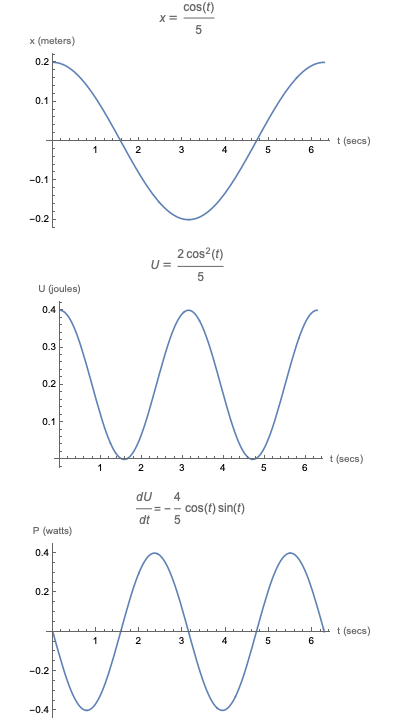
\includegraphics[height=6in]{img/spring}
\end{figure}

\newpage

\begin{theorem}[Chain rule]
If $y=f(u)$ is a differentiable function of $u$ and $u=g(x)$ is a differentiable function of $x$, then 
\begin{equation*}
\frac{\dee y}{\dee x} = \frac{\dee y}{\dee u}\frac{\dee u}{\dee x}
\end{equation*}
or equivalently,
\begin{equation*}
(f\circ g)'(x) = f'(g(x)) g'(x).
\end{equation*}
\end{theorem}

\begin{example}
An object moves along the $x$-axis so that its position at time $t$ seconds is
\begin{equation*}
x(t) = \cos(t^2+1)
\end{equation*}
centimeters.
Compute the velocity of the object for each time $t$.
\end{example}

\newpage

\begin{example}
Differentiate $\sin(x^2+x)$ with respect to $x$.
\end{example}

\vfill

\begin{example}
Find the derivative of $g(t) = \tan(5-\sin 2t)$ with respect to $t$.
\end{example}

\vfill\vfill
\newpage

\begin{example}
Calculate the following.
\begin{enumerate}[label=(\alph*)]
\item $\DS\frac{\dee}{\dee x}\left(5x^4-x^3\right)^7$
\vfill
\item $\DS\frac{\dee}{\dee x}\frac{1}{3x-2}$
\vfill 
\item $\DS\frac{\dee}{\dee x}\sin^5 x$
\vfill 
\end{enumerate}
\end{example}

\newpage

\begin{example}
We already showed that $\DS\frac{\dee}{\dee x}|x| = \frac{x}{|x|}$.
Use the chain rule to give a much shorter proof.
\end{example}
\vfill

\begin{example}
Show that the tangent lines to the curve $y= 1/(1-2x)^3$ all have positive slopes.
\end{example}
\vfill

\newpage

\begin{remark}\,
\begin{itemize}
\item There is a reason why we prefer radians: they are the ``natural" geometric measure of an angle and lead to ``cleaner" formulas.
\item It is important to understand that $\sin x$ and $\sin(x^\circ)$ are different functions.  The first completes a period over any interval of length $2\pi\approx 6.28319$ while the latter requires an interval of length $360$.
\item Similar remarks apply to the 5 remaining trigonometric functions.
\end{itemize}
\end{remark}

\begin{example}
Compute $\DS\frac{\dee}{\dee x}\sin(x^\circ)$.
\end{example}
